Das Paper beschreibt die Sozial Exchange und Market Exchange Kategorien durch die Art und Form der Belohnung die die Konsumenten durch das Mitwirken an den jeweiligen Methoden erhalten. Sozial Exchange Methoden kennzeichnen sich dabei vorallem durch intrinsische Belohnungen wie Spa\ss{} und weniger durch extrinsische wie Geld, obwohl Annerkennung durch andere Personen oder Firmen allerdings nat\"urlich schon eine Rolle spielen k\"onnen. Bei Market Exchange ist es genau anders herum. Es wird aber nicht nur eine Unterteilung der Co-Creation Exchange Formen sondern auch der  Information Formen durch das Paper vorgenommen.
Auf der einen Seite gibt es Methoden die sich mit den Bed\"urfnissen der Kunden, der Need Information befassen. Wenn man weis, was den Kunden zum Kauf motiviert, welche Vorlieben er hat, ... dann kann man das Risiko eine Fehlinvestition reduzieren. Auf der anderen Seite versuchen manche Methoden das Know-How, die Solution Information, welche die Kunden haben, auszun\"utzen. Laut Paper, Information \glqq wie man eine Technologie anwendet um Kundenbed\"urfnisse in Produkte und Dienstleistungen zu verwandeln\grqq. Die Methoden lassen sich durch die zwei Dimensionen anhand einer Matrix veranschaulichen. Es wird f\"ur jedes der vier Matrixfelder eine Methode besprochen: Toolkits f\"ur User Co-Design, die Lead-User Methode, Ideation Contests und Technical Solution Contests.
\pagebreak
\begin{figure}[h!]
	\caption{Zuordnung der Co-Creation Methoden\cite{COCREATION}}
	\centering
		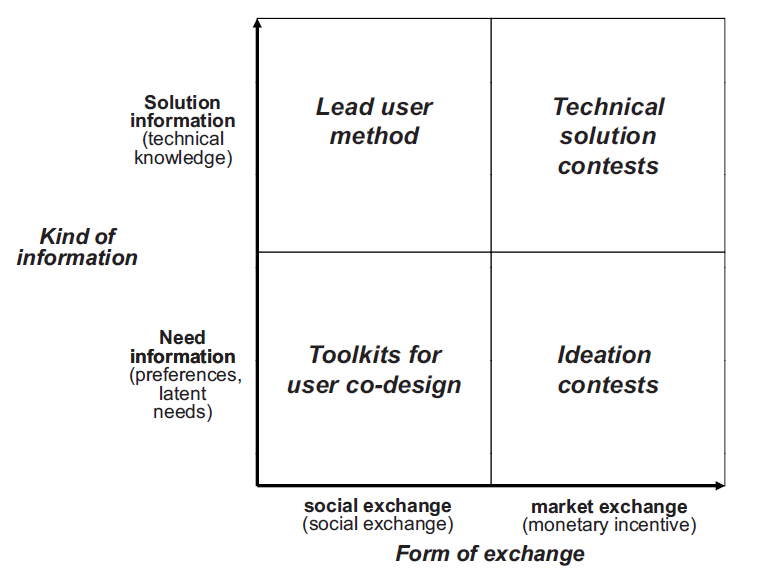
\includegraphics[scale=0.8]{figures/Co-Creation_Matrix}
	\label{quirkyInfluence}
\end{figure}
Das Aufkommen von Sozial Media ver\"andert die Methoden jedoch. Es entstehen neue M\"oglichkeiten aber auch neue Gefahren. Au\ss{}erdem stellt das Paper die These auf, das die Einteilung der Methoden in Exchange Kategorien etwas verschwimmen werden. D.h. bei Market Exchange Methoden werden intrinsische Belohnungen eine gr\"o\ss{}ere Rolle spielen und umgekehrt bei Sozial Exchange Methoden. Als Erstes befassen wir uns mit den Methoden, die sich durch Sozial Exchange kennzeichnen.